% CHAPTER 9: Inference
\chapter{Inference in Transformers}

During the time of prediction, the encoder works in the same way as during training. It generates contextual embeddings for tokens. However, the decoder works \textit{auto-regressively}. It depends on the previous output to generate the next output. Let us see how.

We will be considering a machine translation task in this case. We have to convert the sentence: \textbf{We are friends} to Hindi. Its  translation should be {\devanagarifont हम दोस्त हैं}.

% Input, mask and normalization
\section{The input, masked attention and normalization}

The processing of input, masked multi-head attention and layer normalization are shown below.
\begin{figure}[H]
    \centering
    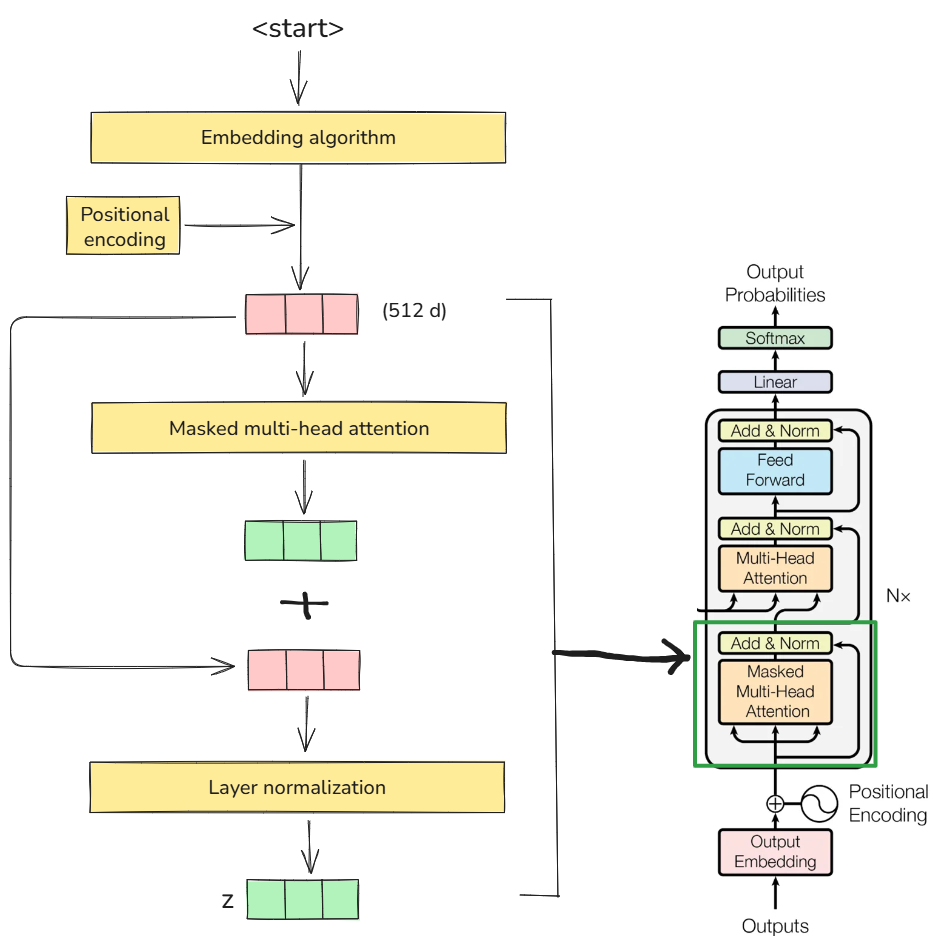
\includegraphics[width=0.5\linewidth]{Decoder-architecture-inference/input-decoder-inference.png}
    \caption{Input, masked attention and layer normalization}
\end{figure}

% Cross-attention
\section{Cross-attention and normalization}

The processing in the cross attention layer is shown below. The key and value vectors are from the encoder, whereas the query vector is from the decoder.
\begin{figure}[H]
       \centering
       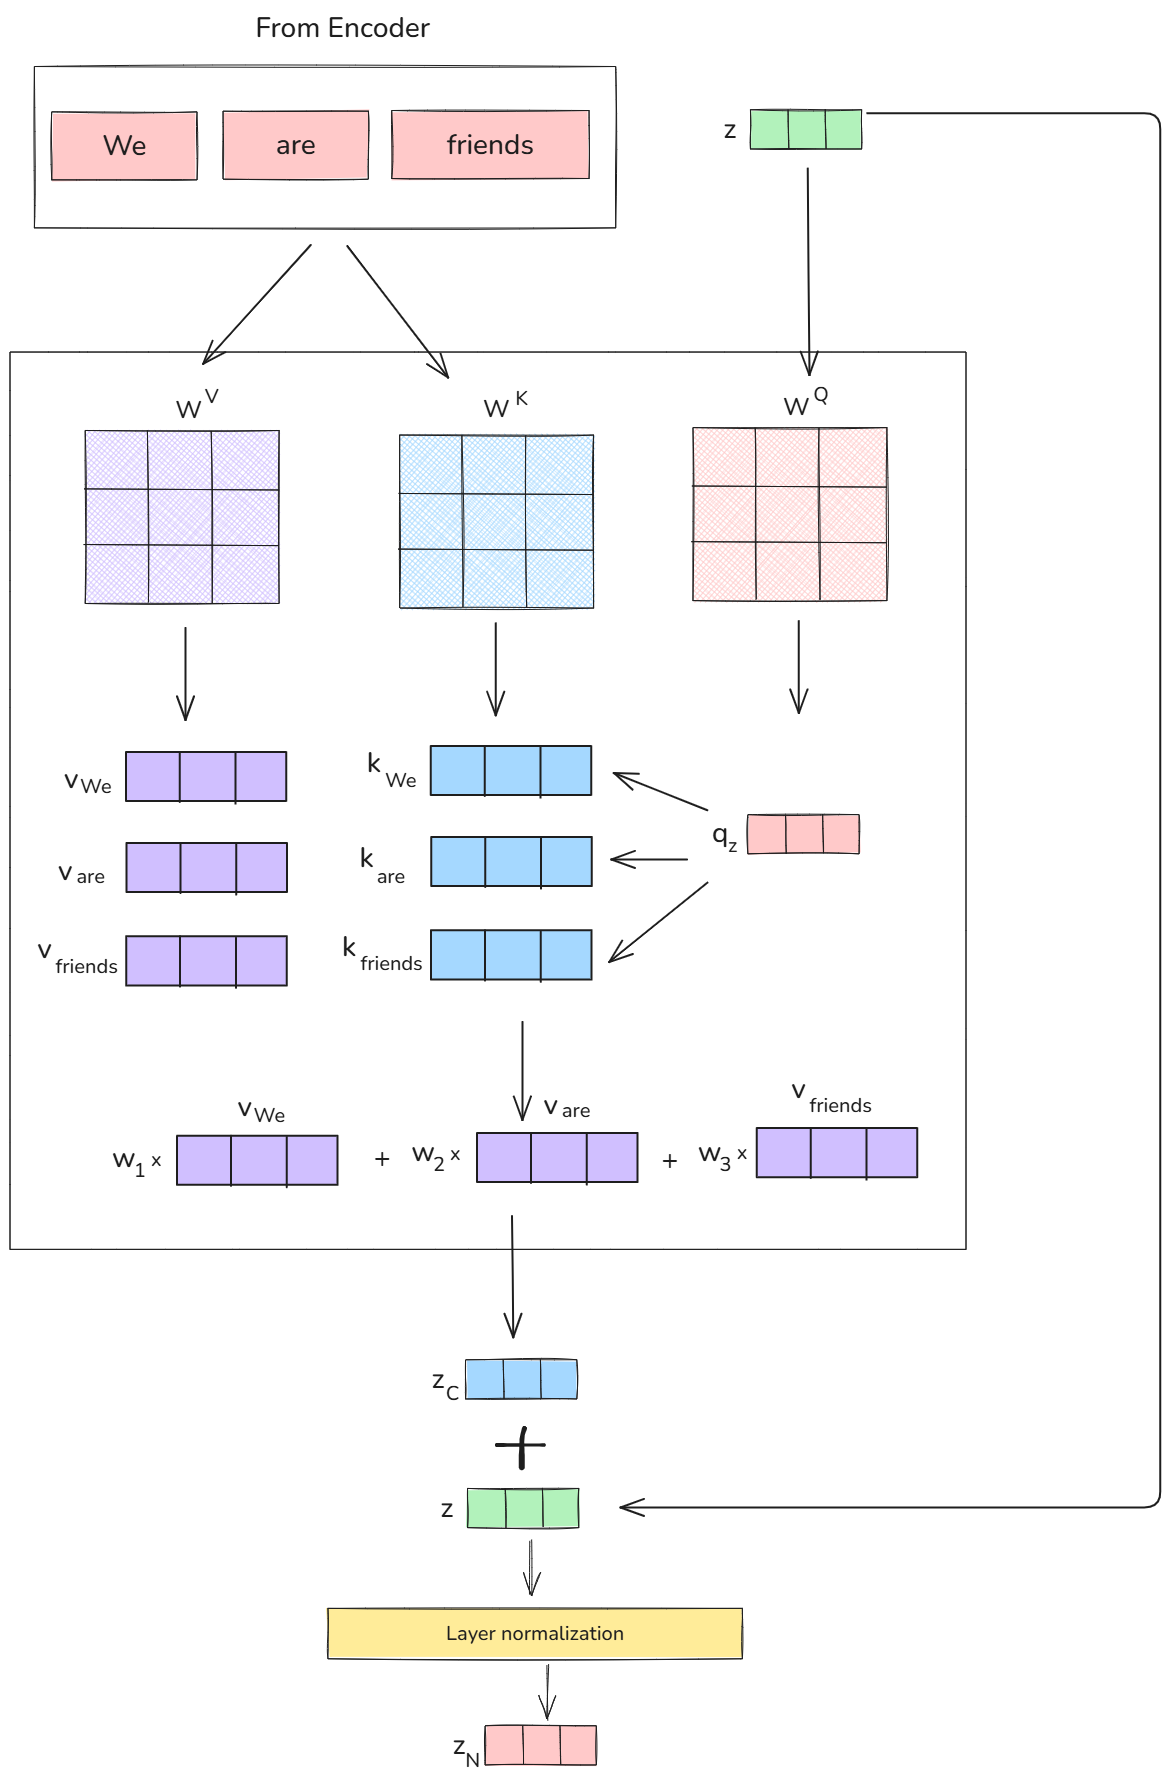
\includegraphics[width=0.5\linewidth]{Decoder-architecture-inference/cross-decoder-inference.png}
       \caption{Cross-attention and layer normalization}
   \end{figure}   

% FFNN
\section{FFNN, normalization and output}

The processing in the subsequent layers is shown. The final output after all the decoder blocks and the output layer is the word {\devanagarifont हम}.
\begin{figure}[H]
    \centering
    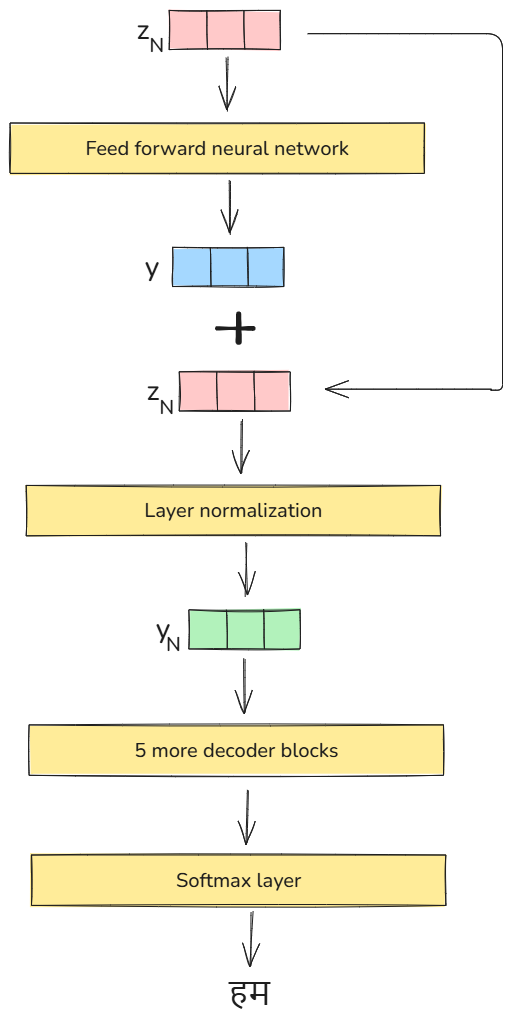
\includegraphics[width=0.3\linewidth]{Decoder-architecture-inference/FFNN-output-decoder-inference.png}
    \caption{FFNN and output block}
\end{figure}

% Inference through timesteps
\section{Subsequent inputs and outputs}

After the prediction of the 1st word, the next input to the decoder is the total output generated till now, i.e., <start> {\devanagarifont हम}. Then the decoder predicts the next word in the sequence and so on. It stops when it predicts a special \textit{<end>} token, which marks the end of the sentence.

Masking is also done during the inference stage in the decoder to ensure that information of future tokens is not available in the present. For example, {\devanagarifont हम} cannot access the embeddings of {\devanagarifont दोस्त} and {\devanagarifont हैं}.
\begin{figure}[H]
    \centering
    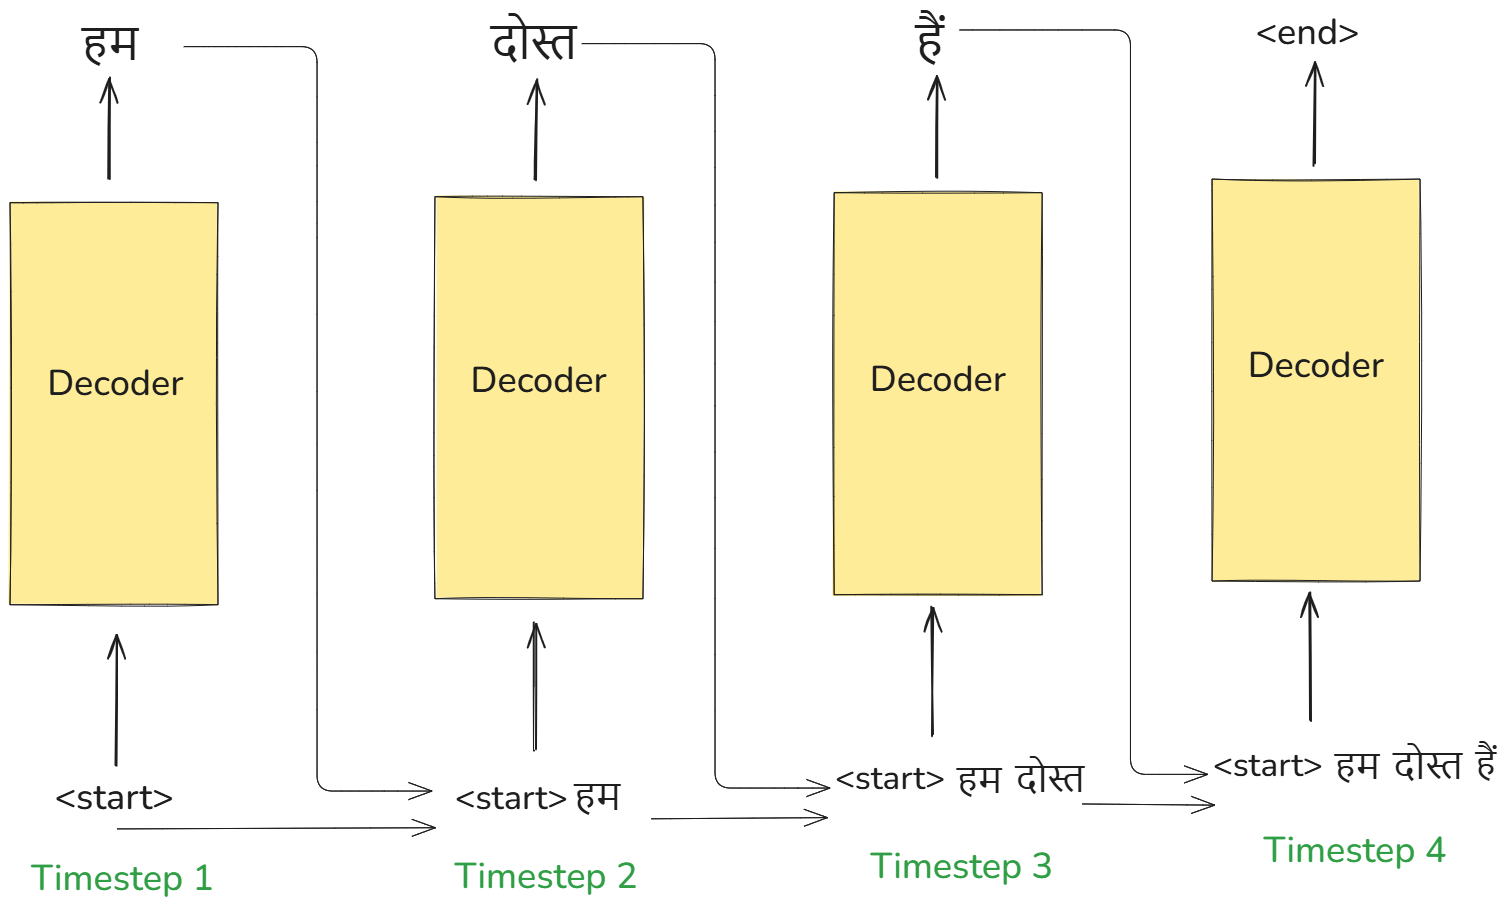
\includegraphics[width=0.5\linewidth]{Decoder-architecture-inference/final-decoder-inference.png}
    \caption{Decoder inference through timesteps}
\end{figure}

